\section{Rat Behavior Model}
\subsection{Preliminaries}
We consider behavioral interaction as a Markov Decision Process (MDP) which is
defined as a 4-tuple $M=\{\mathcal{S},\mathcal{A},\mathcal{P}_a,\mathcal{R}_a\}$,
where $\mathcal{S}$ is a set of states called the state space, $\mathcal{A}$ is
a set of possible actions the robot can take, $\mathcal{P}_a(s,s{'})$ is the
probability that action $a$ in state $s$ at time step $t$ will lead to state
$s{'}$ at time step $t+1$, $\mathcal{R}_a(s,s{'})$ is the immediate reward (or
expected immediate reward) received after transitioning from state $s$ to state
$s{'}'$, due to action $a$ \cite{MDP}. As has been proved in our previous study
\cite{gao-eng-2022, gao-proc}, the state space includes 8 motion primitives and
6 behaviors (Table \ref{table:movement and behavior of rats}). They can be
described as functions of a 3-tuple $\{T,f,\phi\}_s$, where $T$ is the time
duration, $f$ is the motion or behavior frequency and $\phi$ is the amplitude of
the motion or behavior of the state $s$. Accordingly, the action space contains
the transition between each state in the state space. Our aim is to find the
optimal policy at time $t$ to reach the point at where the accumulated
interaction information entropy is less than at elsewhere.
\begin{equation}\label{eq:objective-function}
\begin{aligned}
  &\pi^*(s_1,s_2,a)=\arg\min_{a\in\mathcal{A}}\int I^t(s_1,s_2,a) dt \\
  &\text{s.t.}~I^t(s_1,s_2,a)=\sum_{s_1^{t+1},s_2^t,s_2^{t+1}}p(s_1^{t+1},s_2^t,
  s_2^{t+1})\log_2(\frac{p(s_2^{t+1}|s_1^{t+1}),s_2^t}{s_2^{t+1}|s_2^i})
\end{aligned}
\end{equation}
where $\pi^*$ is the optimal policy given states of the two rats $s_1,~s_2$ and
action $s$ in the format of probability dense function, $I$ is the interaction
information entropy between rats. The details of the interaction information
entropy can be found in \cite{gao-eng-2022, gao-proc}.

\subsection{Behavior Similarity Evaluation}
In Markov Decision Process, the immediate reward should be given as quickly as
possible to the agent so that it can take actions at once to accommodate itself
to the environment. But the value of the interaction information entropy would
not change until the rats enters into the new state after a duration of $T$.
That means an immediate evaluation method to measure the actions in interaction
is required to speed up the decision making. To this end, we use the
well-validated method of representational similarity analysis (RSA) \cite{rsa}
at short timescale to calculate the reward.

Given that both the states and the actions are sequences of animal joints
movements, they can be described as
\begin{equation}\label{eq:motion-description}
\begin{aligned}
  s &=& F_s(\Theta) &= (\Theta_1, \Theta_2, \cdots, \Theta_N)\\
  a &=& F_a(\Theta) &= (\Theta_1, \Theta_2, \cdots, \Theta_n)\\
    &&\Theta&=[\theta_1,\theta_2,\cdots,\theta_7,\nu,\omega]^T
\end{aligned}
\end{equation}
where $\theta_i,~(i=1,2,\cdots,7)$ represents the $i$th joint displacements of the
animal, and $\nu,\omega$ represents the linear and the angular velocity of the
animal with respect to the world frame. $\Theta$ is the motion description
variables in the configuration space of both the robot and the animals.

From Equation (\ref{eq:objective-function}) and Equation (\ref{eq:motion-description}),
we have the expected entropy as
\begin{equation}\label{eq:proof}
  \begin{aligned}
    E{I(s,a)}&=EF(s^{t},s^{t+1},a^t)\\
          &=EF(F_s^{t}, F_s^{t+1}, F_a^{t})\\
          &=EF(F_s^{t}, F_s^{t}p(s^{t+1}|s^t,a^t), F_a^{t})\\
          &=F(EF_s^{t}, EF_s^{t}p(s^{t+1}|s^t,a^t), EF_a^{t})\\
          &=F(F_s^{t}, F_s^{t}Ep(s^{t+1}|s^t,a^t), F_a^{t})\\
          &=F(F_s^{t}, F_s^{t}\sum_{s\in\mathcal{S}}p(s|s^t,a^t), F_a^{t})\\
          &=G(\Theta^t)
  \end{aligned}
\end{equation}

From Equation (\ref{eq:proof}), it can be proved that the expected interaction
information entropy is the function of motion description variables at time $t$,
with no need of future knowledge. Therefore, it is reasonable to use $\Theta$ to
calculate the current immediate reward. As multi-channel measures of motions are
quantitatively related to each other and to computational theory and behavior by
comparing representational dissimilarity matrices, RSA can be seamlessly applied
in this context \cite{RSA-intro}.

To apply RSA, we first calculate the Pearson correlation of the motions between
the policy-generated data and real rats' motion data. Then we calculate the
kinematic similarity matrix at the time step as $M$.

% Since the rats' cognition and decisions
% are affected by the relative positions and the partner's motions, the immediate
% reward in the context of interaction is defined as a function of the motion
% descriptions variables as,

To obtain the probability function $p(s)$ in Equation (\ref{eq:objective-function}),
the open-field test is used to study the spontaneous activities of animals in a
new environment. It allows experimental animals to move freely in a certain
space with few restrictions, and has become an important method to study animal
movements and behaviors \cite{PRUT20033, EILAM200353}. Scientists usually divide
the movements of rats into movements such as going straight, turning, standing
up, and staying in one place. Correspondingly, the behaviors of rats are divided
into behaviors such as exploring, grooming, and resting to reflect the different
activity characteristics of rats\cite{the_rat_study,whishow_bejavior,
MARSHALL2021420,dunn_profiling}. In this paper, we observed the activities of
individual rats (Rattus norvegicus) in a $1{\rm m}\times 1{\rm m}\times 1{\rm m}
$ open field, and marked the key movement joints of rats. Through the records of
10 min a day, we obtained a dataset of the movements of three rats over five
days. The rats involved in this study came from the same litter and were seven
weeks old. The dataset (150 min) contains 3537 rat movements.

Through the observation of rat data, we found that there were some specific
combinations in the movement time series of rats. The frequency of these
combinations is relatively high, which can reflect the activity characteristics
of rats. Therefore, we used a softmax classifier to map the combination of
movements to the behavior, and counted the probability distribution of the
combinations and behaviors. Table \ref{table:movement and behavior of rats} 1
shows the movement and behavior of the rats we observed.
Table \ref{table:relevancy between each movement combination and behavior} shows
the relevancy between each movement combination and behavior (the numbers in
brackets represent the probability). We built the individual pattern of rats on
the basis of the behavior law shown in Table
\ref{table:relevancy between each movement combination and behavior}.
% \begin{table}[b]
%     \caption{Movement and Behavior of Rats}
%     \centering
%     \begin{tabular}{cccc}
%             \hline
%             Movement & Symbol & Behavior & Symbol \\
%             \hline
%             Head pitching & $M_1$ & Sniffing & $B_1$ \\
%             Head yawing & $M_2$ & Exploring & $B_2$ \\
%             Body pitching & $M_3$ & Walking & $B_3$ \\
%             Body yawing & $M_4$ & Trotting & $B_4$ \\
%             Going Straight & $M_5$ & Resting & $B_5$ \\
%             Turning & $M_6$ & Grooming & $B_6$ \\
%             Staying & $M_7$ & & \\
%             Forelimb swing & $M_8$ & & \\
%             \hline
%             \end{tabular}
%     \label{table:movement and behavior of rats}
% \end{table}

\begin{table}[b]
    \caption{Relevancy Between Each Movement Combination and Behavior}
    \centering
    \begin{tabular}{cc}
            \hline
            Movement combination & Behavior \\
            \hline
            Head pitching & $M_1$ \\
            Head yawing & $M_2$ \\
            \hline
            \end{tabular}
    \label{table:relevancy between each movement combination and behavior}
\end{table}

\subsection{Individual Motion Generation}
The interaction between rats will appear in various states, such as tracking,
imitating and contacting. At present, there are still great difficulties in
contact simulation of the robot (insufficient freedom of forelimbs, difficult to
accurately control contact parts and contact forces, etc.). Hence, we avoid
contacting when controlling the robot interaction. When counting the rat
behavior data, the probability of rat contacting is transformed into tracking
and imitating in proportion.

To effectively learn the interactive behavior model between rats, we defined A
as the rat that actively generates the interaction intention and B as the rat
that passively responds to the interaction. Among them, the stimulator (${\rm
R_A}$) executes the individual pattern, and the receiver (${\rm R_B}$) switches
between the individual pattern and the interaction pattern. In the interaction
pattern, the behavior of ${\rm R_B}$ is determined by ${\rm R_A}$. Which pattern
${\rm R_B}$ executes depends on the probability of interaction ($\rm
P_{interaction}$) between two rats, as show in Figure \ref{interaction-process}.
$a_{i+1}$, $b_i$ and $b_{i+1}$ are the behavior of ${\rm R_A}$ at $t_{i+1}$,
${\rm R_B}$ at $t_i$ and ${\rm R_B}$ at $t_{i+1}$ respectively.
\begin{figure}[h]
    \centering
    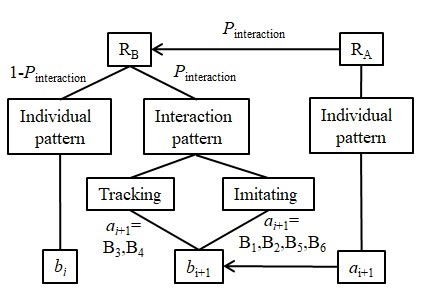
\includegraphics[width=0.8\textwidth]{interaction-process.jpg}
    \caption{The interaction process between $\rm R_A$ and $\rm R_B$.}
    \label{interaction-process}
\end{figure}
Furthermore, we verified the rationality of the proposed strategy. We observed
the interaction process between the rats. We divided three rats, 1, 2 and 3,
into three groups and placed them in a $1{\rm m}\times 1{\rm m}\times 1{\rm m}$
open field in pairs (rats 1 and 2; rats 1 and 3; rats 2 ant 3). Each group
recorded 20-min rat behavior data. During the recording process, the active rat
is always marked as A and the passive rat is marked as B. Then, we obtained
approximately 1000 behavior data of rats A and B, respectively. We counted the
behavior probability distribution of rats A and B in the process of interaction,
and the joint hypotheses test (F-test) was used to verify whether the behavior
probability distribution of rats in the interaction was consistent with that in
the individual pattern. Our results are shown in Table \ref{table:Behavior
Probability Distribution of Rats}. It can be seen that there is no significant
difference between the behavior distribution probability of $\rm R_A$ and that
of individuals, that is, $\rm R_A$ always executes the individual pattern; the
behavior distribution probability of RB is significantly different from that of
individuals, so the behavior of $\rm R_B$ is affected by $\rm R_A$.
\begin{table}[b]
    \caption{Behavior Probability Distribution of Rats}
    \centering
    \begin{tabular}{cccc}
            \hline
            Behavior & Individual & $\rm R_A$ & $\rm R_B$ \\
            \hline
            $\rm B_1$ & 0.015 & 0.05 & 0.1 \\
            $\rm B_2$ & 0.284 & 0.15 & 0.05 \\
            $\rm B_3$ & 0.16 & 0.35 & 0.5 \\
            $\rm B_4$ & 0.167 & 0.15 & 0.05 \\
            $\rm B_5$ & 0.213 & 0.15 & 0.1 \\
            $\rm B_6$ & 0.071 & 0.15 & 0.2 \\
             &  & ${\rm F}=1.67<{\rm F}_{0.05,(5,5)}=5.05$ & ${\rm F}=5.13<{\rm F}_{0.05,(5,5)}=5.05$ \\
            \hline
            \end{tabular}
    \label{table:Behavior Probability Distribution of Rats}
\end{table}

\subsection{Interaction Motion Generation}
